\section{ESF and the recovery step}
\label{sec:method}

We write ESF for the flagging procedure of Algorithm~\ref{alg:adaptive}. Unless stated
otherwise, ESF is followed by the recovery step of Algorithm~\ref{alg:recovery}, and
\emph{ESF alone} denotes Algorithm~\ref{alg:adaptive} without it. The recovery step
(Section~\ref{sec:recovery}) is described after the fit whose flagged set it examines.

\subsection{Exact fits on small subsamples}

For a set $S$ of units, the least-squares clusterwise fit of $S$ solves
\begin{equation}
\min_{z\in\{1,\dots,K\}^{S}}\ \min_{\theta\in\R^{Kd}}\ \sum_{i\in S}\bigl(y_i-x_i^{\top}\theta_{z_i}\bigr)^{2}.
\label{eq:lsfit}
\end{equation}
For fixed labels the inner problem separates into $K$ ordinary least-squares fits, so the
difficulty lies in the labels alone. On the whole sample the problem is hard: whether $n$ points
in the plane can be covered by $K$ lines, that is whether \eqref{eq:lsfit} with one covariate has
value zero, is NP-complete when $K$ is part of the input \citep{megiddo1982complexity}. On a
subsample of a few dozen units it can be solved exactly by a depth-first branch and bound over
label vectors, which prunes a partial labelling as soon as the sum of the residual sums of
squares of its groups exceeds the best value found (Supplement, Section~S7). The cost does not depend on $n$, but it grows quickly with $K$ and $m$ (Supplement,
Table~S30), which limits ESF to a small number of groups.

For fixed coefficients the best label of each unit is its nearest line, so the exact fit of a
subsample is a $K$-means fit with lines in place of centres \citep{pollard1981strong}; here
and below a \emph{line} is the graph of $x\mapsto x^{\top}\theta_k$, a hyperplane when there
is more than one covariate. The same rule, $h_{\theta}(u)=\argmin_k(y-x^{\top}\theta_k)^{2}$ for a unit $u=(x,y)$, with ties
broken by the smallest index, extends the fit to the whole sample. We call the fit of one
subsample a \emph{replicate}; it is \emph{admissible} if each of its $K$ groups contains at
least $d+1$ units, and inadmissible replicates are discarded and redrawn, which forces
$m\pi_{\min}\gtrsim d+1$ for the subsample size $m$ and the smallest group proportion
$\pi_{\min}$.

\subsection{Cost of the exact fit}
\label{sec:solvers}

ESF needs about a hundred solves of \eqref{eq:lsfit} on a dozen units per data set, so what
matters is the cost of one small solve. On the same subsamples we compared our depth-first
search, which also prunes partial labellings that cannot give every group $d+1$ units, with
repetitive branch and bound \citep{brusco2006repetitive} and with the mixed logical-quadratic
programme of \citet{carbonneau2011globally} solved by Gurobi~13.0 \citep{gurobi2026} and by
SCIP~10.0 \citep{maher2016pyscipopt} (Supplement, Section~S4 and Tables~S26 and~S30). For
$m\le20$ the depth-first search was $30$ to $180$ times faster than Gurobi, and further still
than SCIP, which solves a different, big-$M$ formulation of the programme. The gap closes as
$m$ grows, and the programme overtakes the search from about $m=40$ with two groups; the
repetitive bound made the search slower at every size tried. Exactness matters for accuracy less
than for reliability (Section~\ref{sec:intro}; Supplement, Table~S14): with one start of hard
alternation in place of the exact fit, ESF alone lost up to $0.11$ with four groups, and with
elemental fits as in RANSAC up to $0.25$.

\subsection{Sequential flagging}
\label{sec:algorithm}

Algorithm~\ref{alg:adaptive} states ESF. It runs in $L$ stages, each drawing $B/L$ admissible
replicates from the units not yet flagged; after each stage all replicates so far are scored by
a bounded loss on those units, and the units far from the best-scoring replicate are flagged.
The flags are recomputed at every stage, so a unit flagged at one stage can be reinstated at
the next.

\begin{algorithm}[tbp]
\caption{ESF: clusterwise regression from exactly solved subsamples, with sequential flagging}
\label{alg:adaptive}
\begin{algorithmic}[1]
\Require data $(x_i,y_i)_{i\le n}$; number of groups $K$; subsample size $m$; replicates $B$;
stages $L$; weight $\lambda$; cut-offs $c$, $c_{\mathrm b}$
\State $\mathcal F\leftarrow$ units whose covariates are outlying (robust distance above the
$0.975$ quantile of $\chi^{2}_{p}$, $p$ the number of covariates)
\For{$\ell=1,\dots,L$}
  \State draw $B/L$ admissible replicates, on subsamples of size $m$ drawn uniformly from
    $\{1,\dots,n\}\setminus\mathcal F$, each solved exactly
  \State $r_{bi}\leftarrow\min_k(y_i-x_i^{\top}\hat\theta^{(b)}_k)^{2}$, the squared residual
    of unit $i$ from its nearest line of replicate $b$, for every replicate $b$ so far and
    every unit $i$
  \State $s^{2}\leftarrow\min_b\operatorname{med}_{i\notin\mathcal F}r_{bi}/0.4549$, the median
    taken over the unflagged units
    \Comment{$0.4549$ is the median of a $\chi^{2}_1$ variable}
  \State $F_b\leftarrow\sum_{i\notin\mathcal F}\min\{r_{bi},c_{\mathrm b}^{2}s^{2}\}$;\quad
    $w_b\leftarrow\exp\{-\lambda(F_b-\min_{b'}F_{b'})/[(n-|\mathcal F|)\,s^{2}]\}$
  \State reference $\leftarrow$ replicate $b^{\ast}=\argmin_bF_b$
  \State $\mathcal F\leftarrow\{i:\ \text{$i$ is far from the reference in the response or in
    the covariates}\}$ (\emph{Flagging} below)
\EndFor
\State labels $\tilde z\leftarrow$ plurality of the nearest-line labels of all replicates,
  weighted by $w$
\State refit each group on its unflagged units; concentration steps keeping $n-|\mathcal F|$
  units
\State reweighting: recompute the flags at the current fit and refit on the unflagged units
\State \Return coefficients $\hat\theta$, labels $h_{\hat\theta}(u_i)$ for every unit, the flags
  $\mathcal F$ recomputed at $\hat\theta$, and $\hat\alpha=|\mathcal F|/n$
\end{algorithmic}
\end{algorithm}

\emph{Flagging.} A unit is far from a fit $\theta$ in the response if its absolute residual
from its nearest line exceeds $c$ times the scale of the group of that line. That scale is
$1.4826$ times the median absolute residual of the units assigned to the line (or of all
units, when fewer than ten are); with a scale per group, a group with small noise does not
hide outliers and a group with large noise is not trimmed. A unit is far in the covariates if its robust distance from the other
units of its group, computed with the minimum covariance determinant \citep{rousseeuw1999fast},
exceeds the $0.975$ quantile of $\chi^{2}_p$; the test is applied to groups with at least
$\max(10,5p)$ units, and at the start, before any fit, to all units as one group. It is the
covariate trimming of TCLUST-REG \citep{garciaescudero2010robust} with a fixed quantile in
place of a trimming level.

\emph{Scoring.} The bounded loss caps each squared residual at $c_{\mathrm b}^{2}s^{2}$, where
$s$ is a scale common to all replicates, so a replicate that fits the clean units well has a low
score whatever the outliers do. The scale is the smallest, over the replicates, of the median
squared residual over all unflagged units, scaled to estimate the error variance of a
replicate that fits the clean majority (Supplement, Section~S7). The criterion has a weakness
that more search does not cure. With a small group, the
bounded loss with the best replicate's scale can prefer two nearly parallel lines on the large
group, whose units they fit more tightly, to one line on each group, and a wider search finds
such fits more often: with $B=500$ replicates in place of $100$, the cell means of the
small-group designs at $30\%$ of outliers fell by $0.04$ to $0.07$ (Supplement, Table~S29),
and the recovery step then has to undo what the scoring chose. A less biased scale did not
help (Supplement, Section~S6.2).

\emph{Labels and final fit.} The labels of the final fit are the weighted plurality of the
labels that the replicates give to each unit, after alignment with a pilot replicate that
serves only for alignment (Supplement, Section~S7). The concentration steps are those of least
trimmed squares \citep{rousseeuw2006computing} and TCLUST-REG, with the number of retained
units set by the flags rather than by a level, and the last step is the reweighting step of
robust regression \citep{rousseeuw1987robust,gervini2002class}; every unit then receives the
label of its nearest fitted line.

\subsection{Is the flagged set a group?}
\label{sec:recovery}

ESF flags every unit that its $K$ lines do not explain, and it cannot tell a unit that belongs
to no group from a unit of a group it has missed. The second case arises when one group is
small: the best-scoring fit may spend two nearly parallel lines on the large group and flag
most of the small group (Section~\ref{sec:further}; Figure~\ref{fig:illustr}). A trimming
method at a generous level does the same by construction. The recovery step,
Algorithm~\ref{alg:recovery}, examines the flagged set for this case. It uses only a fit
$\hat\theta$, its flagged set $\mathcal F$ and the group scales $s_k$ of the flagging rule, so
it applies after ESF and equally after TCLUST-REG with reweighting. In the
algorithm, $\mathcal F'$ is $\mathcal F$ without the units of the initial covariate screen,
which cannot form a line in the response. The weight $w$ is that of the Gaussian component in
a two-component fit to the residuals of the flagged units near the candidate line; this fit is
the \emph{peak test}.


\begin{algorithm}[tbp]
\caption{The group-recovery step, applied to a fit and its flagged set}
\label{alg:recovery}
\begin{algorithmic}[1]
\Require fit $\hat\theta$ with flags $\mathcal F$ and group scales $s_1,\dots,s_K$; noise range
$R=1.1\,(\max_iy_i-\min_iy_i)$; margin $\tfrac{d+1}{2}\log n$; restriction factor $12$ on the variances
\State stop if $|\mathcal F|>n/3$; otherwise let $\mathcal F'$ be $\mathcal F$ without the units
of the initial covariate screen, and $s=\operatorname{med}_k s_k$
\State fit a line $\beta$ to $\mathcal F'$: the line through $d$ units of $\mathcal F'$, among
$500$ random choices, that has most units of $\mathcal F'$ within $cs$, refitted three times by
least squares on the units within $cs$
\State stop unless at least $\max\{2(d+1),0.03n\}$ units of $\mathcal F'$ lie within $cs$ of
$\beta$ and they form a peak: in the model $w\,\mathcal N(0,s^{2})+(1-w)\,\mathrm{U}(-3cs,3cs)$
for the residuals from $\beta$ of the units of $\mathcal F'$ within $3cs$, the fitted $w$ is at
least $\tfrac12$
\For{$j=1,\dots,K$}
  \State $\theta^{(j)}\leftarrow$ the lines of $\hat\theta$ without line $j$, together with
  $\beta$, refitted by the reweighting step
\EndFor
\State score every fit by the log-likelihood $\ell$ of $K$ Gaussian lines plus a uniform noise
component of density $\pi_0/R$, with the scales, proportions and noise weight
$\pi_0$ read off the fit (the units of the initial covariate screen count as noise)
\State among the $\theta^{(j)}$ whose scales are all at most $\sqrt{12}\,\min_ks_k$, with $s_k$ the scales of $\hat\theta$, take the one
with the largest $\ell$; it replaces $\hat\theta$ if $\ell(\theta^{(j)})-\ell(\hat\theta)$
exceeds the margin
\State apply the step again while the fit changes, at most three times in all
\end{algorithmic}
\end{algorithm}

\begin{figure}[tbp]
\centering
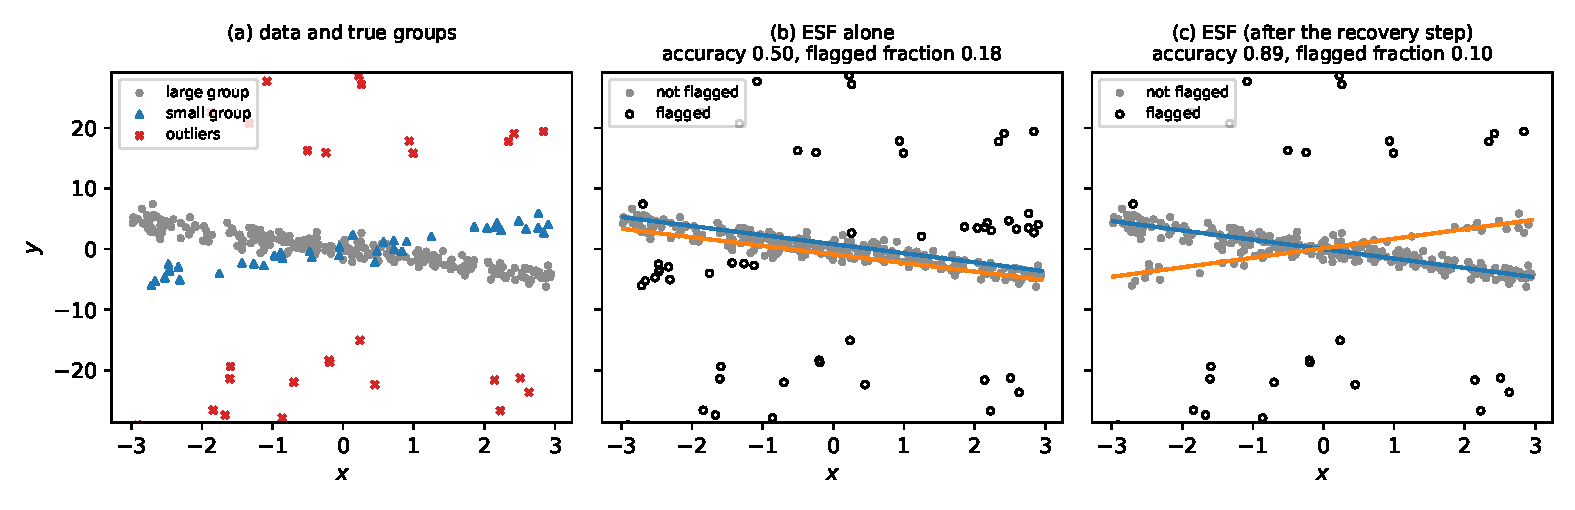
\includegraphics[width=0.9\textwidth]{figures/illustr.pdf}
\caption{The recovery step on one simulated data set of the third part of the study (groups of
$85\%$ and $15\%$ of the clean units, $n=300$, $\varepsilon=0.10$, $28$ outliers). (a) The true
groups. (b) The fit of ESF alone: two nearly parallel lines on the large group, with most of the
small group flagged. (c) After the recovery step. Flagged units lie more than $2.5$ robust
scales from every line.}
\label{fig:illustr}
\end{figure}

The steps have simple reasons. A missing group lies close to one line, so a line is sought
among the flagged units, as in RANSAC \citep{fischler1981random}. Gross outliers also contain
lines that pass near many of them, so most flagged units near a candidate must sit in a peak
of the width of the fitted groups, not in a band.
The comparison uses the likelihood of the model that the flagging rule assumes, Gaussian
groups and flagged units spread over the range of the response: two lines through one group
describe it hardly better than one line, whereas a group of $n_1$ units described as noise
instead of by its own line loses about $n_1\{\log(\pi_1R/\pi_0)-\log\sigma_1-1.42\}$ in
log-likelihood (Proposition~\ref{prop:recover-value}). The noise range $R$ is set by the
extreme responses, so gross outliers raise the value of a group; a range taken over the
unflagged units alone lost small groups (Supplement, Section~S6). The margin is a heuristic
modelled on the Bayesian information criterion. The restriction on the scales of a candidate fit is that of
TCLUST-REG: the factor $12$ bounds the ratio of the group variances, that is $\sqrt{12}$ on
the scales, as in the TCLUST-REG runs of Section~\ref{sec:simulation}, and it prevents a
candidate from absorbing the contamination into a wide group. The peak test does not exclude every band: a band of uniform noise of half-width
below about $3.4$ scales passes it (Supplement, Section~S2.3), and after a generous trimming
level the step accepted such bands at high contamination (Section~\ref{sec:gate2}). The step is
not attempted when a third of the units or more are flagged, because the fit it would examine
is then itself in doubt. The constants are fixed, not fitted to the data
(Section~\ref{sec:constants}).

\paragraph{Relation to trimmed likelihood curves.} The question the step asks, whether the
discarded units hide a group, is the one that classification trimmed likelihood curves
\citep{garciaescudero2011exploring} and the constrained-likelihood approach of
\citet{cerioli2018finding} answer for model-based clustering by fitting the model over a grid
of pairs $(K,\alpha)$ and reading the number of groups and the level off the curves. For
clusterwise regression FSDA's \texttt{tclustregIC} \citep{riani2012fsda,torti2021semiautomatic}
chooses the number of groups and the restriction factor by an information criterion at a
given level, and the level itself is monitored over a grid \citep{torti2019assessing}; the
level is thus still the analyst's choice. The recovery step answers that question locally,
post hoc and for a single candidate: it needs no grid over $\alpha$, and it works after a method that has no $\alpha$, such as ESF
or a reweighted fit; but it tests one candidate at a time, at the $K$ of the fit, and cannot
tell that the fit has one group too many or that the level was too low. When the number of
groups is in doubt, a scan over $K$ such as that of \texttt{tclustregIC} is the better tool,
and the step is then a check on what the chosen level trimmed.

\subsection{Tuning constants and defaults}
\label{sec:constants}

Supplement Table~S44 lists the constants of both algorithms, the values used in every
experiment, the range examined and the largest change in a cell's mean accuracy over that
range. Up to $20\%$ of outliers, moving one constant over its range changed a cell mean by at
most $0.05$, with four exceptions: the loss cap ($0.13$ lost at $c_{\mathrm b}=5$ in D5, while ESF
alone gains $0.24$ with a group of $15\%$ and no outliers, a gain we obtain instead through the
recovery step), the covariate quantile with high-leverage points ($0.21$), the limit on the
flagged fraction ($0.20$ at $0.25n$) and $m=12$ in every design ($0.07$ lost with four groups); $B=500$ replicates moved cell means by $-0.02$ to $+0.03$ up to $20\%$ and
by up to $-0.07$ at $30\%$.


\paragraph{The two constants that stand in for the level.} The subsample size must allow every
group $d+1$ units, so $m\ge(d+1)/\pi_{\min}$; larger values make clean replicates more accurate
but rarer, since a subsample is clean with probability close to $(1-\varepsilon)^{m}$. We used
$m=8$ for two groups and one covariate, $m=10$ when one group has $30\%$ of the units, and
$m=12$ for three groups or three covariates. The default rule is to take $m$ near
$(d+1)/\pi_{\min}$, rounded to an even number, for the lower bound $\pi_{\min}$ on the smallest
group proportion that the analyst is prepared to assume, and $m=12$ when no bound is
available. A lower bound on $\pi_{\min}$ is prior knowledge of the same kind as an upper bound
on $\varepsilon$, and the competitors are not given it, so ESF with $m=12$ in every design was
run on all data sets and appears as a row of Tables~\ref{tab:mainlow}, \ref{tab:level}
and~\ref{tab:mainhigh}. Over the $89$ cells up to $20\%$ of outliers its mean accuracy is
$0.912$ against $0.914$, with the same two cells below $0.85$, and beyond $25\%$ it is $0.813$
against $0.820$. The loss is concentrated in the four-group design ($0.88$ against $0.95$), where
$m=12$ leaves three units per group, and in clustered outliers at $\varepsilon=0.20$ ($0.75$
against $0.78$). With small groups the recovery step makes up for the smaller subsamples, which cost ESF alone
more (mean $0.864$ against $0.874$ over the $89$ cells up to $20\%$; Supplement, Tables~S12, S15, S28 and~S39). The cap of $n/3$ on the
flagged set is a guard against applying the recovery step to a fit that has broken down, not
a trimming level: moving it to $0.25n$ lost $0.16$ and $0.20$ in the two small-group designs
at $\varepsilon=0.20$, where ESF alone flags about a quarter of the units, and moving it to
$0.40n$ gained up to $0.05$ in those designs at $\varepsilon=0.30$ and moved no other cell by
more than $0.01$ (Supplement, Table~S23 and Section~S5). A higher cap is reasonable only when the
contamination is known to be below a third and a small group is suspected.

\paragraph{Other constants.} The vote weight is $\lambda=3$, with $B=100$ replicates in
$L=10$ stages (Section~\ref{sec:stage}). The cut-off $c=2.5$ is the usual value for
reweighting in robust regression \citep{rousseeuw1987robust}: at the true parameter a clean
unit is then flagged with probability $2\Phi(-2.5)\approx0.012$ (Proposition~\ref{thm:step}).
The cap $c_{\mathrm b}=3$ lies slightly above $c$, so that a unit at the flagging boundary
still contributes its full residual.

\paragraph{A default for real data.} The study used $B=100$ replicates and one seed per
data set, and on the fishery data (Section~\ref{sec:fishery}) the answer depended on the seed.
The default for real data is $B=100$ with the best of five seeds by the likelihood of the model
of the recovery step, a rule that returned the modal fit every time on the fishery data and, on
the simulated data, raised cell means up to $20\%$ of outliers and lowered one cell beyond
(Supplement, Section~S6.3). When a group is fitted exactly, as the flat tariff of
Section~\ref{sec:taxi}, the likelihood rewards any line through tied points and the seeds
should be compared by eye. The flagged fraction $\hat\alpha$ is the check on the result. A
value well below any plausible contamination means that the outliers have been absorbed into a
fitted line and the fit has broken down (Section~\ref{sec:high}). A value well above it,
as on the tone and taxi data, means that the errors are not close to Gaussian or that a group's
covariates are compact; $\hat\alpha$ is then not an estimate of the contamination.
